\documentclass[crop,tikz]{standalone}% 'crop' is the default for v1.0, before it was 'preview'=
\usepackage{amsthm}
\usepackage{xspace}

\usetikzlibrary{positioning,calc,arrows,decorations,shapes,decorations.pathreplacing,chains,fit,arrows.meta,intersections,positioning,automata,external,backgrounds}

% \tikzexternalize % activate!
% \makeatletter
% \tikzset{
%   beamer externalising/.style={%
%     execute at end picture={%
%       \tikzifexternalizing{%
%         \ifbeamer@anotherslide
%         \pgfexternalstorecommand{\string\global\string\beamer@anotherslidetrue}%
%         \fi
%       }{}%
%     }%
%   },
%   external/optimize=false
% }
% \makeatother

\tikzset{>=latex}

% \pgfdeclareimage[width=2cm]{enclave}{icons/enclave}
% \pgfdeclareimage[width=2cm]{enclave-yellow}{icons/sgx_red}
% \pgfdeclareimage[width=2cm]{enclave-red}{icons/sgx_yellow}
% \pgfdeclareimage[width=2cm]{server}{icons/server_contoured}
% \pgfdeclareimage[width=2cm]{blockchain}{icons/blockchain}
% \pgfdeclareimage[width=2cm]{user}{icons/persons/user/user}
% \pgfdeclareimage[width=2cm]{attacker}{icons/persons/burglar}
% \pgfdeclareimage[width=1cm]{phone}{icons/smartphone}
% \pgfdeclareimage[width=2cm]{computer}{icons/devices/client}

% \pgfdeclareimage[width=2cm]{memory}{icons/computerpack/013-ram}
% \pgfdeclareimage[width=1.4cm]{gpu}{icons/computerpack/002-vga}
% \pgfdeclareimage[width=1.4cm]{mouse}{icons/computerpack/017-mouse}
% \pgfdeclareimage[width=1.4cm]{keyboard}{icons/computerpack/024-keyboard}
% \pgfdeclareimage[width=1.4cm]{screen}{icons/computerpack/018-monitor-2}
% \pgfdeclareimage[width=1.4cm]{lan}{icons/computerpack/023-lan}
% \pgfdeclareimage[width=1.4cm]{lanred}{icons/computerpack/023-lan-red}

% \definecolor{col1}{RGB}{170, 72, 59}
% \definecolor{col2}{RGB}{170,114, 59}
% \definecolor{col3}{RGB}{ 38, 93,105}
% \definecolor{col4}{RGB}{ 44,127, 66}

\definecolor{col1}{HTML}{4398D1}
\definecolor{col2}{HTML}{FF4842}
\definecolor{col3}{RGB}{ 38, 93,105}
\definecolor{col4}{RGB}{ 44,127, 66}

\definecolor{greenc}{HTML}{64c37d}
\definecolor{redc}{HTML}{e13957}

\ifstandalone
    \newcommand{\icon}[1]{../icons/#1}
\else
    \newcommand{\icon}[1]{images/icons/#1}
\fi

\newcommand{\imgmemory}{
\includegraphics[width=2.0cm]{\icon{computerpack/013-ram}}}
\newcommand{\imggpu}{
\includegraphics[width=1.4cm]{\icon{computerpack/002-vga}}}
\newcommand{\imggpusmall}{
\includegraphics[width=1.0cm]{\icon{computerpack/002-vga}}}
\newcommand{\imgmouse}{
\includegraphics[width=1.4cm]{\icon{computerpack/017-mouse}}}
\newcommand{\imgkeyboard}{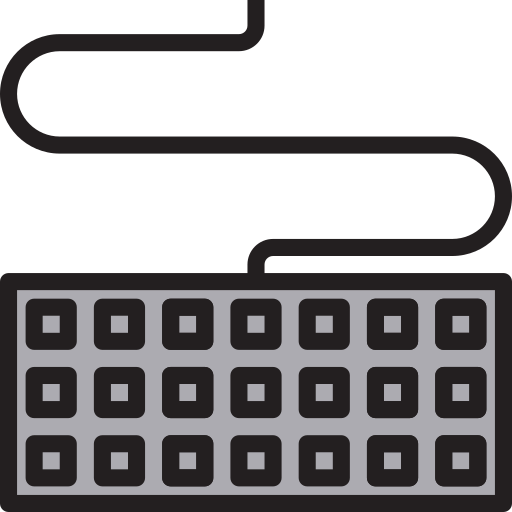
\includegraphics[width=1.4cm]{\icon{computerpack/024-keyboard}}}
\newcommand{\imgscreen}{\includegraphics[width=1.4cm]{\icon{computerpack/018-monitor}}}
\newcommand{\imglan}{
\includegraphics[width=1.4cm]{\icon{computerpack/023-lan}}}
\newcommand{\imglanred}{
\includegraphics[width=1.4cm]{\icon{computerpack/023-lan-red}}}
\newcommand{\imgcpu}{
\includegraphics[width=1.4cm]{\icon{computerpack/034-cpu}}}
\newcommand{\imgcpusmall}{
\includegraphics[width=1.0cm]{\icon{computerpack/034-cpu}}}

\newcommand{\imgdisplay}{
\includegraphics[height=1.4cm]{\icon{computerpack/021-mobile}}}
\newcommand{\imgdisplaysmall}{
\includegraphics[height=1.0cm]{\icon{computerpack/021-mobile}}}
\newcommand{\imgsim}{
\includegraphics[height=1.4cm]{\icon{computerpack/008-sim-card}}}
\newcommand{\imgsimsmall}{
\includegraphics[height=1.0cm]{\icon{computerpack/008-sim-card}}}
\newcommand{\imgsd}{
\includegraphics[height=1.4cm]{\icon{computerpack/011-sd-card}}}
\newcommand{\imgsdsmall}{
\includegraphics[height=1.0cm]{\icon{computerpack/011-sd-card}}}
\newcommand{\imgcamera}{
\includegraphics[width=1.4cm]{\icon{computerpack/035-camera}}}
\newcommand{\imgcamerasmall}{
\includegraphics[width=1.0cm]{\icon{computerpack/035-camera}}}

\newcommand{\imgenclave}{\includegraphics[width=2.0cm]{\icon{enclave}}}
\newcommand{\imgenclavesmall}{\includegraphics[width=1.4cm]{\icon{enclave}}}
\newcommand{\imgenclavesmaller}{\includegraphics[width=1.0cm]{\icon{enclave}}}
\newcommand{\imgenenclavered}{\includegraphics[width=2.0cm]{\icon{sgx_red}}}
\newcommand{\imgenenclaveredsmall}{\includegraphics[width=1.0cm]{\icon{sgx_red}}}
\newcommand{\imguser}{
\includegraphics[height=2.0cm]{\icon{persons/user/user}}}
\newcommand{\imgusersmall}{
\includegraphics[height=1.4cm]{\icon{persons/user/user}}}
\newcommand{\imgattacker}{
\includegraphics[width=2.0cm]{\icon{persons/burglar}}}
\newcommand{\imgattackersmall}{
\includegraphics[height=1.4cm]{\icon{persons/burglar}}}
\newcommand{\imgcomputer}{
\includegraphics[width=2.0cm]{\icon{devices/client}}}

\newcommand{\imglock}{\includegraphics[width=0.3cm]{\icon{lock-icon}}}
\newcommand{\imglocklarge}{\includegraphics[width=0.5cm]{\icon{lock-icon}}}
\newcommand{\imgkeyyellow}{\includegraphics[width=0.5cm]{\icon{key-yellow}}}
\newcommand{\imgkeyred}{\includegraphics[width=0.5cm]{\icon{key-red}}}
\newcommand{\imgkeyblue}{\includegraphics[width=0.5cm]{\icon{key-blue}}}
\newcommand{\imgcertred}{\includegraphics[width=0.5cm]{\icon{certificate-red}}}
\newcommand{\imgcertyellow}{\includegraphics[width=0.5cm]{\icon{certificate-yellow}}}
\newcommand{\imgcertblue}{\includegraphics[width=0.5cm]{\icon{certificate-blue}}}

\newcommand{\imgdevil}{\includegraphics[width=0.6cm]{\icon{devil}}}

\begin{document}
\begin{tikzpicture}[
    icon/.style={rectangle,draw=white!50,fill=white,align=center,minimum height=1.8cm,minimum width=1.8cm},node distance=4cm
]
    \node[icon] (cpu) {\imgenclave};
    \node[icon] (keyboard) [left of=cpu] {\imgkeyboard};

    \coordinate (bus1) at ($(cpu.west)!0.5!(keyboard.east)$);
    \draw[-,thick] (cpu.west) -- ($(bus1)-(-0.2,0)$) -- ($(bus1)-(0,0.2)$);
    \draw[-,thick] (cpu.west) -- ($(bus1)-(-0.28,0)$) -- ($(bus1)-(0,0.28)$);
    \draw[-,ultra thick] ($(bus1)-(0,1.1)$) -- ($(bus1)+(0,1.1)$);
    \draw[-,thick] (keyboard.east) -- ($(bus1)-(0.2,0)$) -- ($(bus1)-(0,0.2)$);
    \draw[-,thick] (keyboard.east) -- ($(bus1)-(0.28,0)$) -- ($(bus1)-(0,0.28)$);

    % \pause
    \node[icon] (gpu) [right of=cpu] {\imggpu};

    \coordinate (bus2) at ($(cpu.east)!0.5!(gpu.west)$);
    \draw[-,thick] (cpu.east) -- ($(bus2)-(0.2,0)$) -- ($(bus2)-(0,0.2)$);
    \draw[-,thick] (cpu.east) -- ($(bus2)-(0.28,0)$) -- ($(bus2)-(0,0.28)$);
    \draw[-,ultra thick] ($(bus2)-(0,1.1)$) -- ($(bus2)+(0,1.1)$);
    \draw[-,thick] (gpu.west) -- ($(bus2)-(-0.2,0)$) -- ($(bus2)-(0,0.2)$);
    \draw[-,thick] (gpu.west) -- ($(bus2)-(-0.28,0)$) -- ($(bus2)-(0,0.28)$);

    \node[draw=none,below=0cm of cpu]  (textcpu) (botcpu) {Processor};
    \node[draw=none] (textkey) at (botcpu -| keyboard) {Keyboard};
    \node[draw=none] (textgpu) at (botcpu -| gpu) {GPU};

    \coordinate (botbus1) at ($(cpu.west)!0.5!(keyboard.east)$);
    \node[draw=none] (textbus1) at (botcpu -| botbus1) {Bus};
    \coordinate (botbus2) at ($(cpu.east)!0.5!(gpu.west)$);
    \node[draw=none] (textbus2) at (botcpu -| botbus2) {Bus};
    
    \coordinate (trust1) at ($(cpu.north)+(0,0.3)$); 
    \coordinate (trust2) at ($(cpu.north)+(0,0.7)$); 
    % \draw[fill=red,opacity=0.3] (trust1 -| keyboard.east) -- (trust1 -| cpu.west) -- (trust2 -| cpu.west) -- (trust2 -| keyboard.east) -- cycle;

    \coordinate[above=0.7cm of cpu] (sep);
    \draw[-,dashed,thick] (sep -| keyboard.west) -- ++(5.9,0) -- node[below,align=right,text width=4cm] {Hardware Components} node[above,align=right,text width=4cm] {Logical Entities} (sep -| gpu.east) ; 


    \coordinate[above=1.1cm of sep] (log1);
    \coordinate[above=1.2cm of log1] (log2);
    \node[draw,minimum height=0.6cm] (app1) at ($(log2)-(0.7,0)$) {Encl};
    \node[draw,minimum height=0.6cm] (app2) at ($(log2)+(0.7,0)$) {Encl};
    \node[draw,minimum height=0.6cm,minimum width=2.3cm] (os) at ($(log1)$) {OS};
    \node[draw,minimum height=0.6cm] (per1) at (log1 -| keyboard) {Firmware};
    \node[draw,minimum height=0.6cm] (per2) at (log1 -| gpu) {Firmware};

    \draw[<->,thick] (app1) -- (os.north -| app1);
    \draw[<->,thick] (app2) -- (os.north -| app2);

    \draw[<->,thick] (per1) -- (os);
    \draw[<->,thick] (per2) -- (os);

    % \def\x{0.13};
    % \draw[thick] ($(app1.north east)+(\x,\x)$) -- ($(app1.south east)+(\x,-\x)$) -- ($(per1.south west)+(-\x,-\x)$) -- ($(per1.north west)+(-\x,\x)$) -- cycle node[above,midway] {Platform-wide enclave};
    % \draw[thick] ($(app2.north west)+(-\x,\x)$) -- ($(app2.south west)+(-\x,-\x)$) -- ($(per2.south east)+(\x,-\x)$) -- ($(per2.north east)+(\x,\x)$) -- cycle node[above,midway] {Platform-wide enclave};

    \node[draw=none] at ($(app1.south east)$) {\imglocklarge};
    \node[draw=none] at ($(app2.south east)$) {\imglocklarge};

    % \begin{scope}[on background layer]
    %     \draw[draw=none,fill=red!30] (textkey.south west -| keyboard.west) -- (per1.north west -| keyboard.west) -- (app1.north -| textbus1.south east) -- (textbus1.south east) -- cycle;
    %     \draw[draw=none,fill=red!30] (textgpu.south east -| gpu.east) -- (per2.north east -| gpu.east) -- (app2.north -| textbus2.south west) -- (textbus2.south west) -- cycle;
    % \end{scope}

    % \node[draw=none] at ($(per1.south east)-(0,0.1)$) {\imgdevil};

    % \node[draw=none] at ($(keyboard.north east)+(0.4,-0.1)$) {\imgdevil};
    % \node[draw=none] at ($(keyboard.north east)+(0.4,1.5)$) {\imgdevil};
\end{tikzpicture}
\end{document}
